
\section{Overview}\label{sec:overview}
We introduce a model that explains most concurrency attacks we studied. 
Leveraging the model, we design a framework \xxx
to detect concurrency attacks. 
This section introduces some preliminaries, 
makes an overview of the model and architecture of \xxx, 
and gives an example of how we employ our framework to exploit a concurrency attack. 

\subsection{Preliminary}\label{sec:preliminary}

\emph{\textbf{Input}} To ease discussion, we use input to broadly refer to the data a program
reads from its execution environment, including not only the
data read from files and sockets, but also command line arguments,
return values of external functions such as gettimeofday, and any
external data that can affect program execution

\emph{\textbf{Bug-inducing input}} The inputs that trigger a concurrency bug. 

\emph{\textbf{Attack-inducing input}} The inputs that trigger a concurrency attack.

\emph{\textbf{Attacker thread}} The threads employed by attackers to race other thread.

\emph{\textbf{Infected thread}} The threads raced by attacker thread. In some case, a thread 
can be both infected and victim.

\emph{\textbf{Victim thread}} The threads where attacks happen. In some case, a thread 
can be both infected and victim.


\subsection{Concurrency Attack Model}\label{sec:model}



\begin{figure}
	\centering
	% \vspace{-.1in}
	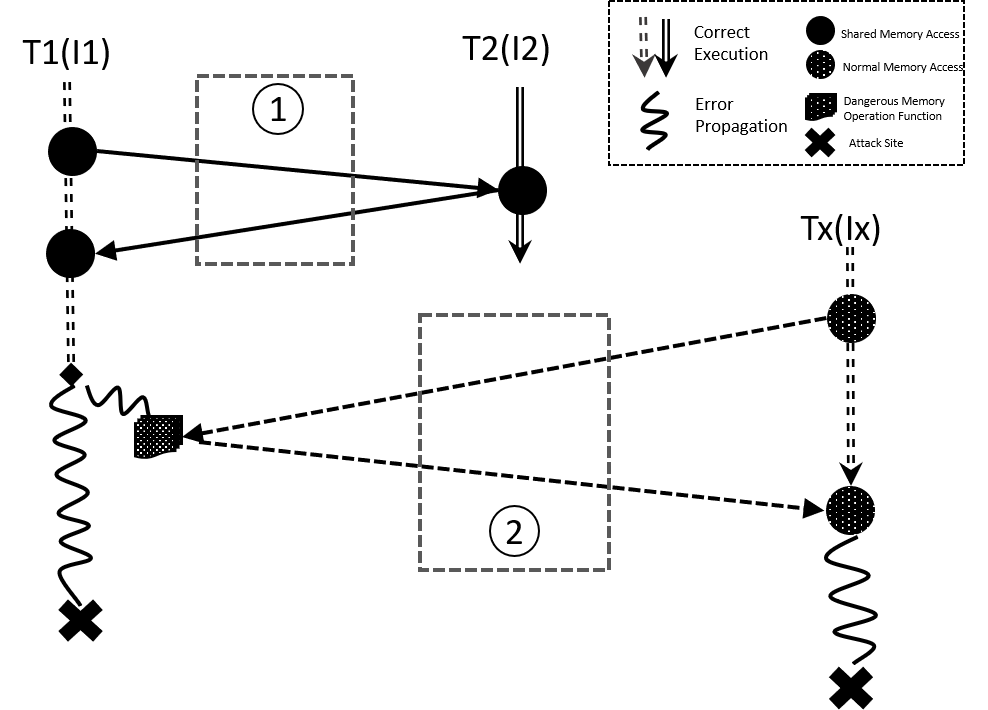
\includegraphics[width=1\columnwidth]{figures/model}
	\vspace{-.25in}
	\caption{{\em Concurrency Attack Model}} 
	\label{fig:model}
	\vspace{-0.1in}
\end{figure}




\subsection{\xxx's Architecture}\label{sec:archi}
\begin{figure*}
	\centering
	% \vspace{-.1in}
	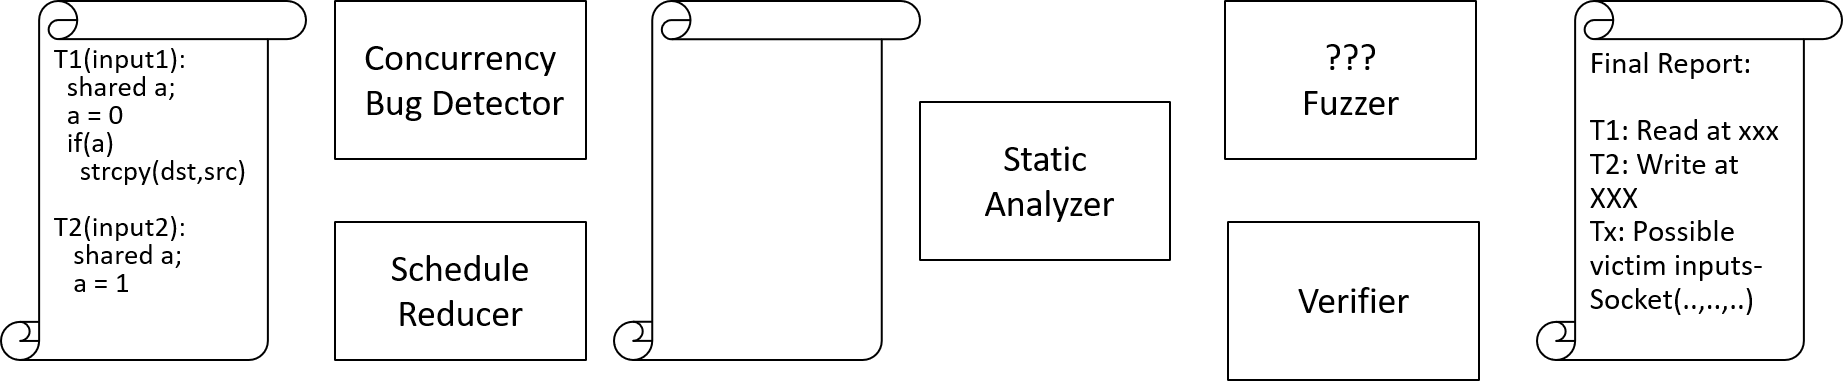
\includegraphics[width=1.8\columnwidth]{figures/archi}
	\vspace{0in}
	\caption{{\em Architecture}} 
	\label{fig:archi}
	\vspace{-0.1in}
\end{figure*}



\emph{\textbf{Concurrency bug detector}} wraps existing concurrency bug detection tools and detects concurrency bugs.  
It receives program executables and inputs, and produces runtime concurrency bug reports. 
Data race detectors are mature for detecting concurrency bugs in industry and has been widely deployed and studied. 
We adopt current popular data race detector includes \tsan, \valgrind, \ski and \ktsan(\S\ref{sec:implementation}).


\emph{\textbf{Schedule Reducer}} reduces benign schedules (\eg, adhoc synchronization), and verifies real concurrency bug happening.  
It receives concurrency bug reports and program IR file, and produces eliminated concurrency bug reports. 
We take static analysis approach to and leverage the runtime information from bug reports, 
which is much simpler and more precise than prior static adhoc synchronization identification tool SyncFinder\cite{syncfinder:osdi10}.

\emph{\textbf{Intra-procedural Static Analyzer}} does inter-procedural static analysis to 
see whether corrupted memory may propagate to 
any vulnerability sites (\S\ref{}) through data flow or control flows. 
Also, it give hints for potential intra-procedural propagation (\eg, heap overflow). 
It receives eliminated concurrency bug reports and program IR file, and produces vulnerability reports.  
We introduces a static analysis algorithm and combines runtime results from concurrency bug detectors to produce  
precise and scalable vulnerability reports and input hints. 

\emph{\textbf{Inter-procedural Fuzzer}} finds potential inputs running on victim thread 
that can be corrupted by intra-procedural propagation(\eg, heap overflow). It receives 
hints from intro-procedural static analyzer, target program executables and crowd-sourced 
benchmarks. It produces hints for potential victim inputs. 
   
  

  

\subsection{Detecting Example}\label{sec:example}

